\chapter{Diseño e implementación} % Main chapter title
En este capítulo se exponen las tomas decisiones relacionadas al diseño e implementación relacionada al hardware y firmware a lo largo del desarrollo del trabajo. 
\label{Chapter3} % Change X to a consecutive number; for referencing this chapter elsewhere, use \ref{ChapterX}

\definecolor{mygreen}{rgb}{0,0.6,0}
\definecolor{mygray}{rgb}{0.5,0.5,0.5}
\definecolor{mymauve}{rgb}{0.58,0,0.82}

%%%%%%%%%%%%%%%%%%%%%%%%%%%%%%%%%%%%%%%%%%%%%%%%%%%%%%%%%%%%%%%%%%%%%%%%%%%%%
% parámetros para configurar el formato del código en los entornos lstlisting
%%%%%%%%%%%%%%%%%%%%%%%%%%%%%%%%%%%%%%%%%%%%%%%%%%%%%%%%%%%%%%%%%%%%%%%%%%%%%
\lstset{ %
  backgroundcolor=\color{white},   % choose the background color; you must add \usepackage{color} or \usepackage{xcolor}
  basicstyle=\footnotesize,        % the size of the fonts that are used for the code
  breakatwhitespace=false,         % sets if automatic breaks should only happen at whitespace
  breaklines=true,                 % sets automatic line breaking
  captionpos=b,                    % sets the caption-position to bottom
  commentstyle=\color{mygreen},    % comment style
  deletekeywords={...},            % if you want to delete keywords from the given language
  %escapeinside={\%*}{*)},          % if you want to add LaTeX within your code
  %extendedchars=true,              % lets you use non-ASCII characters; for 8-bits encodings only, does not work with UTF-8
  %frame=single,	                % adds a frame around the code
  keepspaces=true,                 % keeps spaces in text, useful for keeping indentation of code (possibly needs columns=flexible)
  keywordstyle=\color{blue},       % keyword style
  language=[ANSI]C,                % the language of the code
  %otherkeywords={*,...},           % if you want to add more keywords to the set
  numbers=left,                    % where to put the line-numbers; possible values are (none, left, right)
  numbersep=5pt,                   % how far the line-numbers are from the code
  numberstyle=\tiny\color{mygray}, % the style that is used for the line-numbers
  rulecolor=\color{black},         % if not set, the frame-color may be changed on line-breaks within not-black text (e.g. comments (green here))
  showspaces=false,                % show spaces everywhere adding particular underscores; it overrides 'showstringspaces'
  showstringspaces=false,          % underline spaces within strings only
  showtabs=false,                  % show tabs within strings adding particular underscores
  stepnumber=1,                    % the step between two line-numbers. If it's 1, each line will be numbered
  stringstyle=\color{mymauve},     % string literal style
  tabsize=2,	                   % sets default tabsize to 2 spaces
  title=\lstname,                  % show the filename of files included with \lstinputlisting; also try caption instead of title
  morecomment=[s]{/*}{*/}
}


%----------------------------------------------------------------------------------------
%	SECTION 1
%----------------------------------------------------------------------------------------
\section{Hardware}
\subsection{Construcción de la válvula de control}
\label{subsec:Construcción de la válvula de control}
Para la fabricación del prototipo fue preciso mecanizar una pieza la cual es una caja desmultiplicadora de fuerza que controla una válvula mediante la energización de un servomotor paso a paso. 
Al emplear una válvula de control fue importante estudiar sus características de funcionamiento. 
La válvula es un mecanismo que permite regular el flujo  o caudal, en este caso de agua, entre dos partes del sistema. 
Básicamente la válvula es un ensamblaje compuesto de un cuerpo con conexión a una tubería y de un obturador operado por accionamiento, donde su función principal es variar el caudal del fluido que circula a través de ella, comportándose como un orificio cuya área está continuamente variando. Las válvulas son uno de los instrumentos de control esenciales en la industria.
Debido a su diseño y materiales, las válvulas pueden abrir y cerrar, conectar y desconectar, regular, modular o aislar un enorme  flujo de líquidos y gases.
El obturador determina la característica de caudal de la válvula; es decir, la relación que existe entre la posición del obturador y el caudal de paso del fluido.
El obturador de una válvula, conforme se va desplazando, produce un área de pasaje que posee una determinada relación característica entre la fracción de carrera de la válvula y el correspondiente caudal que escurre a través de la misma. A esa relación se le da el nombre de característica “inherente” de caudal de válvula.
En este trabajo se utilizó una válvula cuya característica inherente es “Tipo de Apertura Rápida”.
Se trata de una característica que produce una variación grande de caudal a través de la válvula con una carrera pequeña. Este tipo de válvula posibilita el pasaje de casi la totalidad del caudal nominal con apenas una abertura de 25 porciento de la carrera total.
Produce una ganancia muy alta a bajas aperturas de carrera y una ganancia muy baja en aperturas por encima de 60 porciento de carrera total. 
La siguiente figura muestra la curva típica de una válvula de apertura rápida.
\begin{figure}[h]
\centering
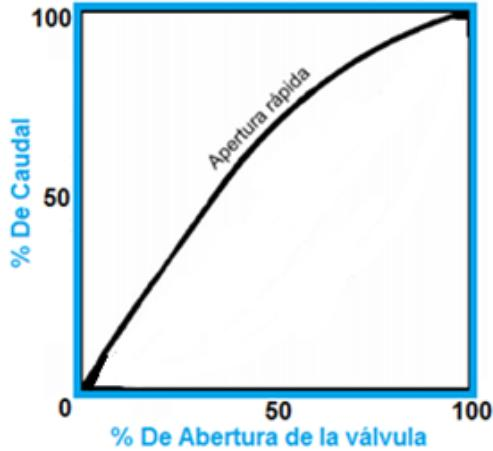
\includegraphics[scale=.50]{./Figures/funcion-valvula.jpeg}
\caption{Gráfica del caudal en función de la apertura de la válvula.}
\label{fig:grafica caudal vs. caudal}
\end{figure}

\subsection{Servomotor}
\label{subsec:Servomotor}
Para el control de la válvula fue necesario un motor que pueda producir un momento de 1 Nm o más. Para este proyecto, por cuestión de disponibilidad, se utilizó un motor paso a paso y un controlador cuyo modelos son 86HS85 y MA860H respectivamente.
El motor paso a paso de 8 hilos posee un torque nominal de 8,5 Nm, suficiente como para realizar movimientos de apertura parcial o total y cierre total de la carrera de dicha válvula, según las necesidades requeridas de caudal. 
El driver MA860H es un controlador para motores paso a paso compatibles con motores 86HS85 con las siguientes características principales:

\begin{enumerate}
	\item Permite ajustar la corriente que se dirige hacia el motor.
	\item Posibilita controlar al motor hasta en 200 micropasos.
	\item Frecuencia de entrada de tren de pulso hasta 300khz. 
	\item Corriente de salida hasta 7.2A.
	\item Entrada TTL compatible y ópticamente aislada.
	\item Soporta modos PUL / DIR y CW / CCW.
\end{enumerate}
El MA860H tiene dos conectores, el conector P1 para conexiones de señales de control y el conector P2 para conexiones de potencia y motor. 
\subsubsection{Configuraciones del conector P1}
PUL+,PUL-: Señal de pulso: esta entrada representa la señal de pulso, activa en cada flanco ascendente o descendente (para este trabajo se encuentra activo en flanco ascendente); 4-5V equivale a un pulso alto y 0-0.5V a un pulso bajo. Para una respuesta confiable, el ancho de pulso debe ser superior a 1,5 microssegundos. 
DIR+;DIR- : Señal DIR: esta señal tiene niveles de voltaje bajo / alto, que representan dos direcciones de rotación del motor. Para una respuesta de movimiento confiable, la señal DIR debe estar por delante de la señal PUL por lo menos 5 microsegundos. 4-5V cuando DIR-HIGH, 0-0.5V cuando DIR-LOW. 

ENA+;ENA-: Señal de Habilitación: esta señal se utiliza para habilitar/deshabilitar el controlador. Nivel alto (la señal de control NPN, PNP y las señales de control diferencial son por el contrario, es decir, nivel bajo para habilitar) para habilitar al controlador y nivel bajo para inhabilitar al controlador.
\subsubsection{Circuito interfaz del conector de señal de control (P1)}
El controlador MA860H puede aceptar entradas diferenciales y de un solo extremo (incluida la salida de colector abierto y PNP). El MA860H tiene 3 entradas lógicas aisladas ópticamente que están ubicadas en el conector P1 para aceptar señales de control del microcontrolador. Estas entradas están aisladas para minimizar o eliminar los ruidos eléctricos acoplados a las señales de control del variador. En la siguiente "Figura \ref{fig:circuito interfaz}", se ilustra las conexiones a colector abierto.
\begin{figure}[h]
\centering
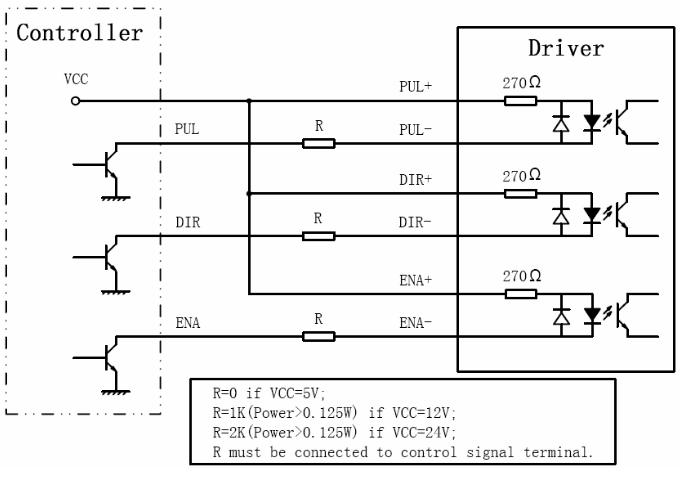
\includegraphics[scale=.65]{./Figures/circuitointerfaz-driver.jpeg}
\caption{Circuito Interfaz - conexiones de señales a colector abierto.}
\label{fig:circuito interfaz}
\end{figure}
Siguiendo las recomendaciones del fabricante relacionadas a la construcción del circuito interfaz entre el diver y el microcontrolador se diseñó y fabricó el circuito eléctrico que se muestra en la "Figura \ref{fig:esquemático circuito interfaz}".

\begin{figure}
\centering
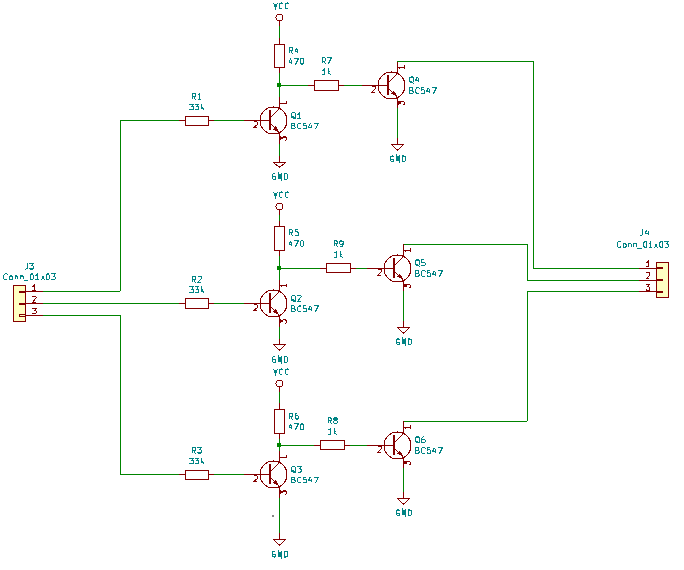
\includegraphics[scale=.85]{./Figures/esquematico-circuito-interfaz.png}
\caption{Esquemático de Circuito Interfaz entre el microcontrolador y driver.}
\label{fig:esquemático circuito interfaz}
\end{figure}

En el esquemático se puede observar dos etapas, la primera es un circuito negador y la segunda corresponde al circuito de colector abierto NPN.
Por todo lo descrito se puede decir que la etapa de potencia está formada por el circuito interfaz y el controlador del motor paso a paso. 
Es importante mencionar que además del motor paso a paso, la electroválvula está constituida por un sensor resistivo de ángulo, que se encuentra adosado al eje de la válvula. La señal derivada de dicho sensor también es retroalimentada y ofrece una estimación de la posición del obturador de la misma. El sensor resistivo es un potenciómetro de una vuelta de 50K ohm cuyo modelo es 91A-503, Bourns cermet.
En la "Figura \ref{fig:Diagrama en bloque de la celda primaria}", podemos observar un diagrama en bloque general que indica entre otras partes del trabajo, cómo está constituido el servomotor.  

\begin{figure}
\centering
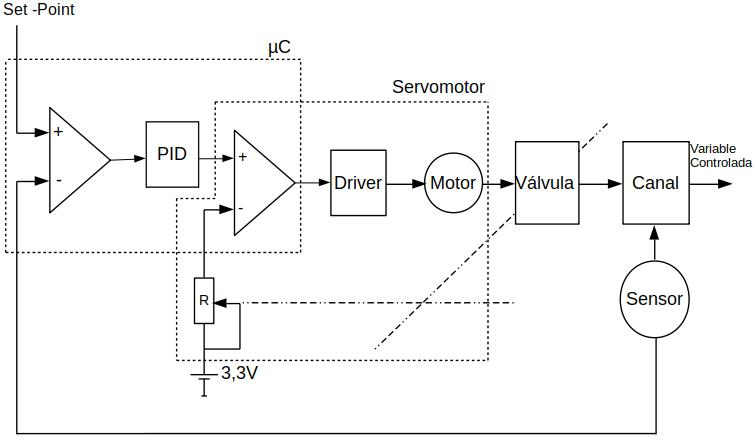
\includegraphics[scale=.65]{./Figures/Diagrama-en-bloque-general-con-servomotor-V2.jpg}
\caption{Diagrama en bloque de la celda primaria.}
\label{fig:Diagrama en bloque de la celda primaria}
\end{figure}
\subsection{Medidor de caudal}
\label{subsec:Medidor de caudal}
La medición del agua es la cuantificación del caudal de agua que pasa por la sección transversal de un río, canal o tubería. También se le conoce como aforo. 
En la mayoría de los casos, la medición del agua resulta de la necesidad de brindar mayor control sobre su uso y distribución. Dicha medición se realiza a través de medidores de caudal. Estos son dispositivos que utilizan diferentes principios mecánicos o físicos para permitir que un flujo de agua pueda ser cuantificado. 
El medidor, que determina la cantidad de fluido que pasa por unidad de tiempo por una sección dada, utilizado en este trabajo para la verificación de caudal de agua proporcionado y además para generar la señal de realimentación correspondiente, es un “Medidor de caudal de Canal Abierto Tipo Aforo”.
Existen varias formas de aforo en canales abiertos, dentro de las principales se encuentran:
\begin{enumerate}
	\item Método volumétrico.
	\item Vertederos.
	\item Canal Parshall. 
	\item Método hidráulico.
\end{enumerate}
Para efectuar el presente trabajo se utilizó el tipo de aforo con vertedero triangular con escotadura en V.
La medición del caudal de las corrientes naturales nunca puede ser exacta debido a que el canal suele ser irregular y por lo tanto es irregular la relación entre nivel y caudal. Los canales de corrientes naturales están también sometidos a cambios debidos a erosión o depósitos. Se pueden obtener cálculos más confiables cuando el caudal pasa a través de una sección donde esos problemas se han limitado. Los vertederos pueden ser definidos como simples aberturas, sobre las cuales un líquido fluye. El término se aplica también a obstáculos en el paso de la corriente y a las excedencias de los embalses. Los vertederos son orificios sin el borde superior y ofrecen las siguientes ventajas en la medición del agua: 

\begin{itemize}
\item Se logra con ellos precisión en los aforos 	
\item La construcción de la estructura es sencilla
\item No son obstruidos por materiales que flotan en el agua 
\item La duración del dispositivo es relativamente larga
\end{itemize}
Los vertederos son utilizados, intensiva y satisfactoriamente en la medición del caudal de pequeños cursos de agua y conductos libres, así como en el control del flujo en galerías y canales.
Para la construcción del vertedero triangular empleado, se precisó de una chapa de hierro plana de 1 mm de espesor, a la que se le  realizó una hendidura de sección triangular, cuyo  valor de ángulo es de 18 grados.
Esta chapa supera los límites del ancho del canal de forma que, ubicándola  verticalmente y en forma transversal al canal, opera como un embalse que por su hendidura sale un flujo de agua.
De esta forma se puede medir en distintos lugares del recorrido del canal, cuál es el caudal real que está pasando por ese punto en particular.  
La "Figura \ref{fig:Placa de aforo}",  muestra la vista de frente de una estructura de un vertedero con escotadura en V. 	
\begin{figure}
\centering
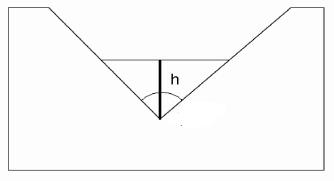
\includegraphics[scale=.85]{./Figures/PlacaDeAforo.jpeg}
\caption{Placa de aforo: vista de frente.}
\label{fig:Placa de aforo}
\end{figure}
La "Figura \ref{fig:Placa de aforo-VistaLateral}", ilustra la vista lateral del vertedero y cómo fluye el líquido por su abertura.
\begin{figure}
\centering
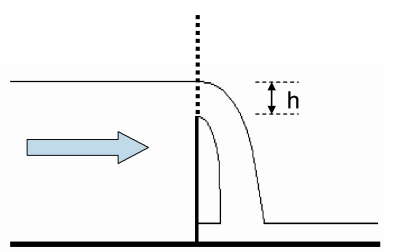
\includegraphics[scale=.85]{./Figures/PlacaDeAforo-VistaLateral.png}
\caption{Placa de aforo: vista lateral.}
\label{fig:Placa de aforo-VistaLateral}
\end{figure}
Entonces, para el calcular el caudal se debe tener en cuenta la siguiente fórmula:
\begin{equation}
 \label{eq:caudal}
 Q = \frac{8}{15}\sqrt{2g} c \tan\alpha  H^\frac{2}{5} 
\end{equation}
	
\begin{figure}
\centering
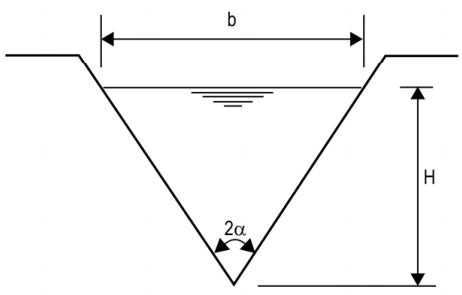
\includegraphics[scale=.75]{./Figures/DimensionesPlacaAforo.png}
\caption{Placa de aforo: dimensiones.}
\label{fig:Placa de aforo dimensiones}
\end{figure}	

Teniendo en cuenta la ecuación \ref{eq:caudal}
\begin{itemize}
\item Q: es caudal en m3/seg
\item g: coeficiente de gravedad
\item c: coeficiente de descarga
\item alpha: ángulo del vertedero
\item H: nivel de agua en metros

\end{itemize}

Los medidores de caudal con aforo triangular como el utilizado en el presente trabajo, responden a una ecuación del modelo que se expone arriba y la misma se obtuvo empíricamente. En el caso de este proyecto y por tratarse de un prototipo a escala, es un medidor que se usará por única vez, por lo tanto la tabla de calibración del caudalímetro fue obtenida experimentalmente.  
En la "Figura \ref{fig:alturas vertedero}", se detalla la vista de frente del canal con el vertedero triangular y los diversos niveles de altura que se consideraron al momento de realizar las mediciones pertinentes. 

\begin{figure}
\centering
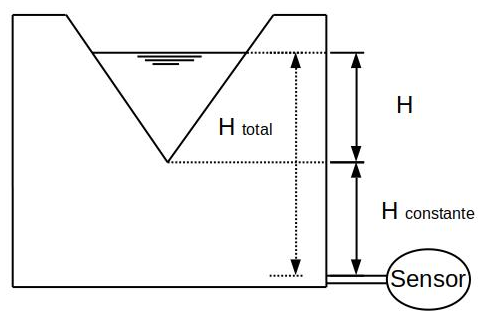
\includegraphics[scale=.75]{./Figures/AlturaVertedero.png}
\caption{Placa de aforo: dimensiones.}
\label{fig:alturas vertedero}
\end{figure}
A partir de la "Figura \ref{fig:alturas vertedero}", se intenta especificar que existe una manguera, la cual uno de sus extremos se conecta a la base del canal y el otro a una de las dos espigas del sensor. Además, se puede advertir los niveles de altura que se deben tener en cuenta. H total corresponde a la altura entre el nivel de agua en un instante dado y la manguera conectada al sensor, H constante se encuentra asociada al nivel de altura que está comprendido entre dicha manguera y el vértice del triángulo del vertedero, y finalmente H variable es la altura que está contenida entre el nivel de agua y el vértice del triángulo de dicho vertedero.    
Por lo tanto, este caudalímetro de canal abierto por sistema de aforo utiliza como medidor de nivel de columna de agua un sensor de presión cuyo modelo es MPX5010DP. 
Este transductor piezo-resistivo, es un sensor de presión de silicio monolítico que puede ser utilizado en aplicaciones que disponen de un microcontrolador o microprocesador con entradas ADC.
El MPX5010DP entrega a su salida un rango de voltaje entre 0v y 5v, mediante esta información y una fórmula que se expone en el siguiente párrafo se puede estimar la presión hasta un valor de 10 KPa, esto es, una columna de agua de hasta 100 cm de altura.
Esta señal proveniente del sensor en conjunto con un algoritmo de control PID, permite regular el caudal de agua en un determinado valor preestablecido. 
El dispositivo proporciona una salida lineal como puede se observar en la "Figura \ref{fig:función de salida del sensor}", extraída de su hoja de datos.

\begin{figure}
\centering
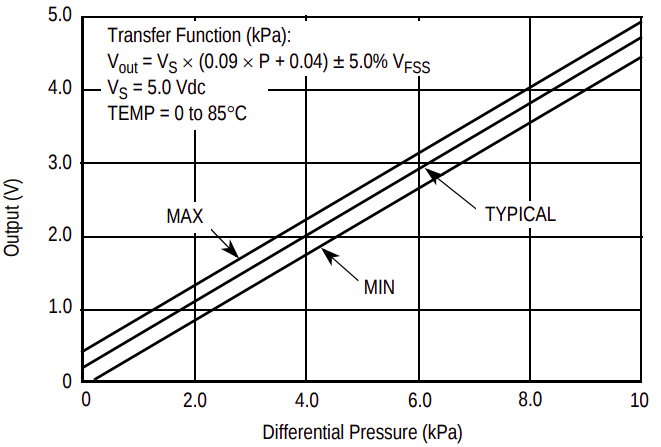
\includegraphics[scale=.55]{./Figures/SalidaMPX5010DP.png}
\caption{Función de salida del sensor de presión MPX5010DP.}
\label{fig:función de salida del sensor}
\end{figure}
Como se pudo observar el gráfico anterior de la "Figura \ref{fig:función de salida del sensor}", la ecuación para obtener la presión del sensor viene dada por la ecuación \ref{eq:presion}:
\begin{equation}
 \label{eq:presion}
 P = \frac{Vout- 0.04*Vs \pm Tol}{0.09*Vs}
\end{equation}
Vs es el valor de voltaje de alimentación Vs = 5v, Vout es el valor de voltaje que entrega el sensor, Tol es la tolerancia, un ajuste que se debe aplicar al sensor para  calibrar a medida.
Tomando como base la ecuación de presión diferencial que relaciona la altura se resuelve que (recordando que la presión a la atmósfera es cero):  

\begin{equation}
 \label{eq:presión}
	 P =PH -PL= P = gh =\frac{Vout- 0.04*Vs \pm Tol}{0.09*Vs}	
\end{equation}
 Donde P es la presión,  es la densidad del agua, g es la gravedad y h es el nivel de la columna líquida.

La disposición de los pines del dispositivo lo podemos advertir en la "Figura \ref{fig:disposición de pines del sensor}":
\begin{figure}
\centering
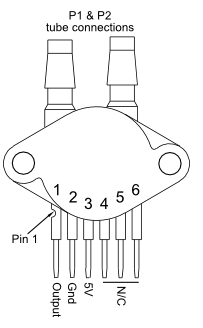
\includegraphics[scale=.65]{./Figures/DisposicionDePinesSensor.png}
\caption{Disposición de pines del sensor de presión MPX5010DP.}
\label{fig:disposición de pines del sensor}
\end{figure}

Siendo la densidad del agua =1000 kgm3  y la gravedad g=10ms2
La ecuación resultante para obtener h es: h=Pg. 
Una vez construido el prototipo, se realizó una calibración de caudal obteniéndose una tabla Caudal vs Htotal (altura). Por lo que, en el firmware esta tabla es utilizada para obtener el valor de caudal  en lugar de la fórmula presentada.
\section{Software}
\subsection{Arquitectura de software}
\label{subsec:Arquitectura de software}

Durante la definición de la arquitectura de software se seleccionaron dos arquitecturas de software y se integraron para confeccionar una arquitectura híbrida, de modo tal que se adapte a las necesidades concretas de este proyecto. Por un lado, se seleccionó una arquitectura en capas, la cual está conformada por tres capas claramente definidas.
En la capa HAL se encuentran los drivers encargados de abstraer los detalles de acceso al hardware. De esta forma, facilitará la migración a otro microcontrolador en caso de que en el futuro hiciese falta. Adicionalmente, permite una mayor claridad en la implementación, separando los drivers de la lógica de la aplicación.
Debido a que en producción se utilizará como hardware a la CIAA-NXP y durante el desarrollo la EDU-CIAA-NXP, se empleó el firmware de la CIAA versión 3.0 como capa de abstracción de hardware. 
En la capa de aplicación se encuentran todos los componentes que encapsulan la lógica de aplicación, y finalmente, la tercera corresponde al sistema operativo de tiempo real. En esta capa se empleó el sistema operativo FreeRTOS.
El sistema incluye sensores que proveen información relacionada al ámbito a controlar y un actuador que cambian dicho ámbito. Por lo tanto, en respuesta a las alteraciones identificadas por los sensores, se envían señales de control a los actuadores del sistema. Entonces, al identificar que dicho sistema debe poseer este tipo de comportamiento se definió emplear una arquitectura de tiempo real inherente al “Control Ambiental”, ya que este patrón de arquitectura de software brinda la posibilidad de recopilar datos del entorno por medio de sensores como así también el estado en el que se encuentran los actuadores  conectados al sistema. Con base en datos reunidos de sensores y actuador, se envían señales de control hacia el actuador para producir cambios en dicho entorno controlado. En la "Figura \ref{fig:Arquitectura de software}", se puede ver el diagrama del patrón arquitectónico que es la base del diseño del sistema de control, y además utilizado en la capa aplicación. 

\begin{figure}
\centering
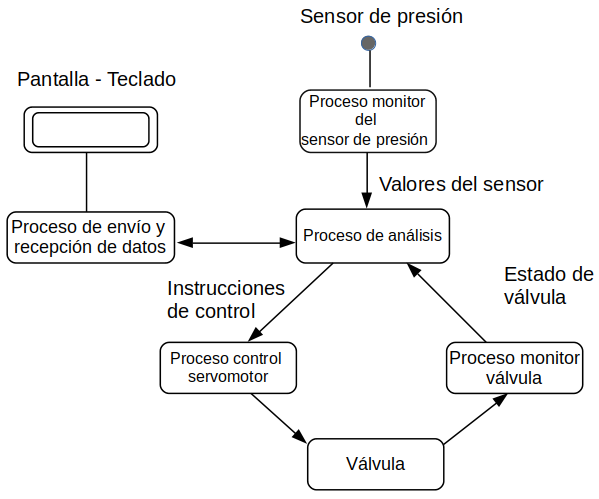
\includegraphics[scale=.65]{./Figures/ArquitecturaSoftware.png}
\caption{Arquitectura de sistema de control de caudal de agua en canal a cielo abierto.}
\label{fig:Arquitectura de software}
\end{figure}

Al aplicar ambos patrones se constituyó un patrón híbrido de dos capas. La capa inferior es la capa de abstracción de hardware. La capa superior, pertenece a la aplicación.

\subsection{Componentes de software}
\label{subsec:Componentes de software}
Cada capa de software es considerada un componente de software. Con lo cual se poseen los siguientes componentes:

\begin{itemize}
\item HAL
\item Sistema Operativo
\item Aplicación
\end{itemize}

A su vez, la capa de aplicación está compuesta por los siguientes componentes de software:

\begin{itemize}
\item Monitor sensor de presión.
\item Control servomotor.
\item Monitor válvula.
\item Control de recepción y envío de datos.
\end{itemize}

En la "Figura \ref{fig:Capas de componentes de software}", se puede apreciar el nivel de jerarquía de cada una de las capas siendo la capa HAL la  más baja: 

\begin{figure}
\centering
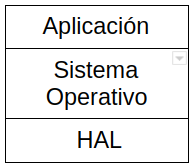
\includegraphics[scale=.75]{./Figures/JerarquiaDeCapas-Software.png}
\caption{Jerarquía de componentes de software.}
\label{fig:Capas de componentes de software}
\end{figure}
\subsubsection{Diseño detallado}
A continuación se incluye el diseño detallado de cada uno de los componentes de software presentados en la "Figura \ref{fig:Arquitectura de software}".
	\begin{figure}
	\centering
	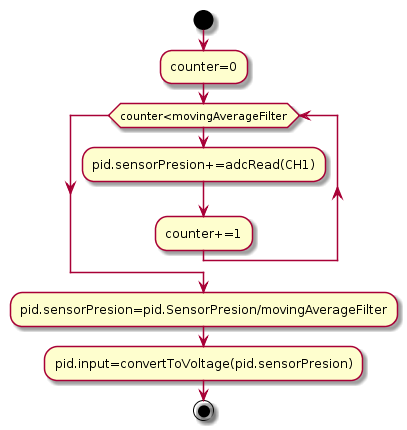
\includegraphics[scale=.65]{./Figures/Procesomonitorsensordepresion.png}
	\caption{Proceso monitor del sensor de presión.}
	\label{fig:Control servomotor}
	\end{figure}
	
\begin{figure}
	\centering
	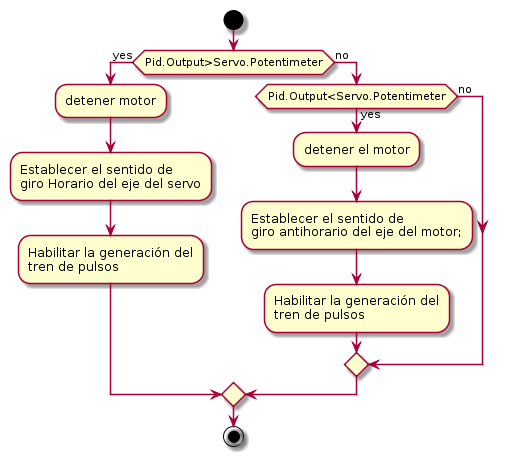
\includegraphics[scale=.55]{./Figures/ProcesoControlServo.png}
	\caption{Proceso de control del servomotor.}
	\label{fig:Control servomotor}
	\end{figure}

 	\begin{figure}
	\centering
	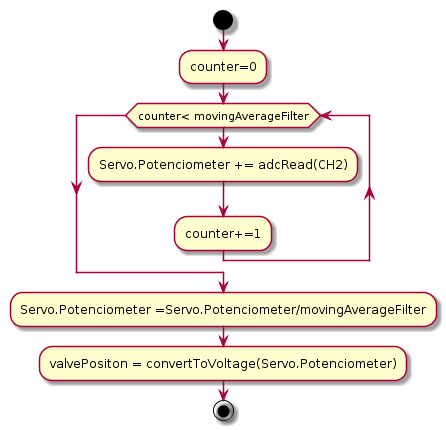
\includegraphics[scale=.65]{./Figures/MonitorValvula.png}
	\caption{Proceso monitor válvula.}
	\label{fig:Proceso monitor valvula}
	\end{figure}

	\begin{figure}
	\centering
	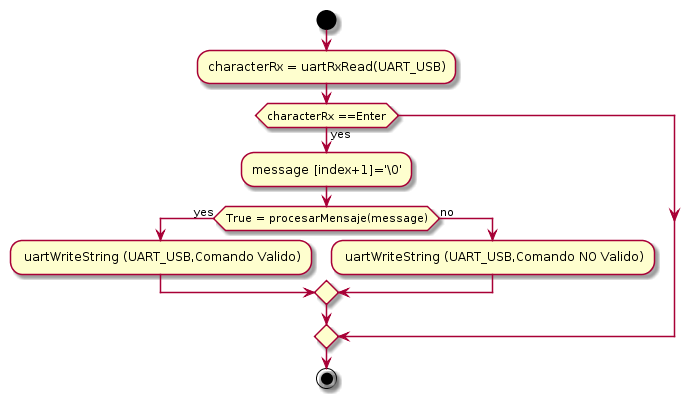
\includegraphics[scale=.65]{./Figures/Porcesorecepcionyenviodedatos.png}
	\caption{Proceso de envió y recepción de datos.}
	\label{fig:Proceso De envió y recepción de datos}
	\end{figure}

	
\begin{figure}
	\centering
	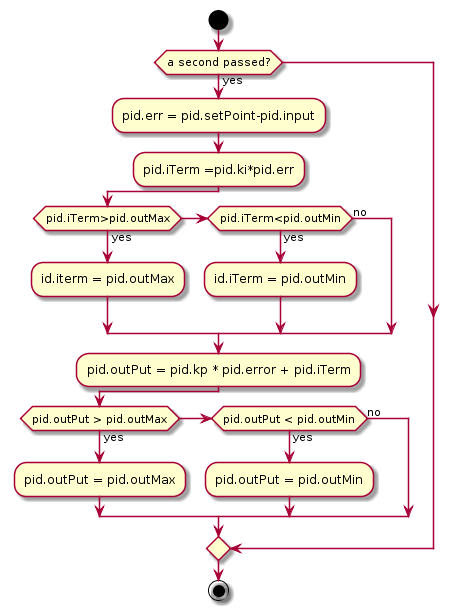
\includegraphics[scale=.65]{./Figures/procesocontrolPID.png}
	\caption{Proceso de Control PID.}
	\label{fig:Proceso de Control PID}
	\end{figure}
\subsection{Casos de uso}
\label{subsec:Casos de uso}
Para la etapa de captura de requerimientos funcionales que el sistema debía satisfacer se emplearon casos de uso correspondientes al Lenguaje Unificado Modelado (UML) ya que es de mucha utilidad y permite especificar, visualizar, construir y documentar los requisitos del sistema especialmente en sistemas con un alto grado de interacción hombre/máquina. A continuación se presentan dos casos de uso considerados como principales.

\subsubsection{Caso de uso: detectar el nivel de agua del canal}
\begin{table}[t]
\begin{center}
\begin{tabular}{ | m{4cm} | m{9.5cm} | }
\hline Nombre & Detectar el nivel de agua del canal \\ \hline
1.1 Breve descripción & 
El firmware debe detectar por medio del sensor de presión el nivel de agua existente en el canal. \\ \hline

 1.2 Actor Principal&La aplicación móvil.\\ \hline


 1.3 Disparadores & La recepción de un comando. \\ \hline

Flujo de Eventos& \\ \hline

 2.1 Flujo básico &
El firmware recibe el paquete desde un smartphone  o desde una aplicación de comunicación serial desde una pc. \\ \hline


 2.1.2 Flujo básico &
El firmware deberá desencapsular el comando recibido y extraer los diferentes campos de información. \\ \hline

 2.1.3 Flujo básico &
El firmware deberá identificar el tipo de operación. \\ \hline


 2.1.4 Flujo básico &
El firmware deberá leer un pin configurado como adc asociado al sensor de presión un valor digital. \\ \hline
 

2.1.5 Flujo básico &
Se repite el paso 2.1.4 hasta 5 veces, de forma que el firmware deberá realizar una acumulación de los valores obtenidos. \\ \hline


2.1.6 Flujo básico &
 El firmware con base al acumulador obtenido en el punto anterior deberá, realizar un filtro de promedio móvil.  \\ \hline
 
2.1.7 Flujo básico &
El firmware deberá convertir el valor digital promediado a tensión. \\ \hline 
2.1.8 Flujo básico &
El firmware deberá obtener el nivel de agua con el dato obtenido en el punto anterior empleando una tabla que se obtendrá experimentalmente. \\ \hline
2.1.9 Flujo básico &
El firmware deberá controlar si el resultado se encuentra dentro de las dimensiones establecidas. \\ \hline
2.1.10 Flujo básico &
El firmware deberá enviar por el puerto serial el valor de nivel de agua en cm. \\ \hline
2.2 Flujo alternativo &  \\ \hline


2.2.1 Flujo alternativo  & 
2.1.9 Si la distancia obtenida se encuentra fuera de rango se enviará por la UART “Distancia Fuera de Rango - Verificar el correcto Funcionamiento del  sensor”. \\ \hline

Requisitos Especiales & \\ \hline


Pre - condiciones & \\ \hline
 
4.1 Pre - condiciones & 
El firmware debe estar en estado de correcto funcionamiento. \\ \hline

4.2 Pre - condiciones &
La comunicación serial se debe encontrar en condiciones óptimas para su funcionamiento correcto. \\ \hline

Post- Condiciones &
El firmware deberá quedar operativo y en correcto 
funcionamiento y en condiciones para la recepción de futuros comandos. \\ \hline

\end{tabular}
\caption{ Caso de uso: detectar el nivel de agua del canal.}
\label{tab:coches}
\end{center}
\end{table}

\subsubsection{Caso de uso:establecer un determinado valor de caudal.}

\begin{table}[t]
\begin{center}
\begin{tabular}{ | m{4cm} | m{9cm} | }
\hline 
Nombre & Establecer un determinado de valor de caudal.\\ \hline
1.1 Breve descripción &
El firmware debe establecer un caudal mediante la manipulación de la posición de la válvula de control.\\ \hline
 1.2 Actor Principal & La aplicación móvil.\\ \hline
 1.3 Disparadores & La recepción de un comando \\ \hline
Flujo de Eventos & \\ \hline


 2.1 Flujo básico &
El firmware recibe el paquete desde un smartphone  o desde una aplicación de comunicación serial desde una pc. \\ \hline
 2.1.2 Flujo básico &
El firmware deberá desencapsular el comando recibido y extraer los diferentes campos de información. \\ \hline
 2.1.3 Flujo básico &
El firmware deberá identificar el tipo de operación. \\ \hline


 2.1.4 Flujo básico &
El firmware deberá leer un pin configurado como adc asociado al sensor de presión un valor digital. \\ \hline


2.1.5 Flujo básico &
Se repite el paso 2.1.4 hasta 5 veces, de forma que el firmware deberá realizar una acumulación de los valores obtenidos.\\ \hline
2.1.6 Flujo básico &
 El firmware con base al acumulador obtenido en el punto anterior deberá, realizar un filtro de promedio móvil.  \\ \hline
2.1.7 Flujo básico & 
El firmware deberá convertir el valor digital promediado a tensión.  \\ \hline
2.1.8 Flujo básico & 
El firmware deberá obtener el caudal con el dato obtenido en el punto anterior empleando una tabla que se obtendrá experimentalmente. \\ \hline
2.1.9 Flujo básico &
El firmware deberá comparar este resultado de caudal obtenido con el set point. \\ \hline
2.1.10 Flujo básico &
En caso de ser valores diferentes, el firmware deberá generar un tren de pulsos hasta posicionar la válvula de control. \\ \hline
2.1.11 Flujo básico &
Se repite desde 2.1.4 hasta que el caudal obtenido a través del sensor y el set point sean iguales. \\ \hline
2.2 Flujo alternativo & \\ \hline


2.2.1 Flujo alternativo & 
2.1.10 Si los valores son iguales el firmware deberá detener la generación del tren de pulsos. \\ \hline
Requisitos Especiales & \\ \hline


Pre - condiciones & \\ \hline
 
4.1 Pre - condiciones &
El firmware debe estar en estado de correcto funcionamiento. \\ \hline
4.2 Pre - condiciones &
La comunicación serial se debe encontrar en condiciones óptimas para su funcionamiento correcto. \\ \hline
Post- Condiciones &
El firmware deberá quedar operativo y en correcto funcionamiento y en condiciones para la recepción de futuros comandos.\\ \hline
\end{tabular}
\caption{ Caso de uso: establecer un determinado valor de caudal.}
\label{tab:establecer un determinado valor de caudal.}
\end{center}
\end{table}

\subsection{Diagrama de clase}
\label{subsec:Diagrama de clase}
Al momento de desarrollar el firmware, de forma previa se realizó un diagrama de clase, que se puede ver en la "Figura \ref{fig:Diagrama de clase.}". 
\begin{figure}
	\centering
	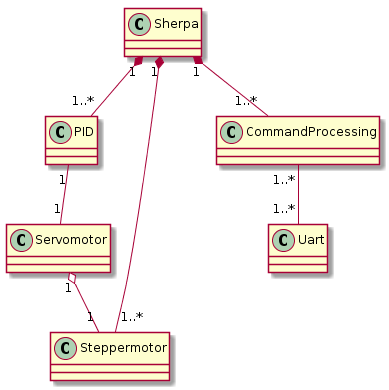
\includegraphics[scale=.75]{./Figures/DiagramaDeClase-DistribucionDeAgua.png}
	\caption{Diagrama de clase.}
	\label{fig:Diagrama de clase.}
	\end{figure}

Uart:  
este módulo recibe y envía los comandos desde y hacia la aplicación de comunicación serial que se ejecuta en la PC.

Command Processing:
acumulará y convertirá de carácter a decimal los comandos recibidos y los devuelve cuando sea solicitado



Stepper Motor:
este módulo posee todas las funciones inherentes al control del motor paso a paso. Interactúa con el módulo Servomotor para integrar las características de un servomotor convencional. 

Servomotor:
el propósito de Servomotor es establecer la posición de la válvula realizando una comparación entre el resultado que se va obteniendo del algoritmo de control PID, output y la posición actual de dicha válvula.

PID:  
este módulo implementa un algoritmo de control PID. El mismo es ejecutado cada un segundo para cuantificar el error o desviación que existe entre el valor de caudal medido a través del sensor de presión y el valor deseado. Este valor es solicitado por el módulo Servomotor.
\subsection{Protocolo de comunicación}
\label{subsec:Protocolo de comunicación}
Se definió un paquete de datos  para que el usuario pueda testear todos los comandos que involucre el servomotor y verificar su correcto funcionamiento. A continuación se detalla lo siguiente:
\begin{enumerate}
\item Habilitar o deshabilitar el motor.
\item Establecer los micro pasos (MicroStep).
\item Establecer el sentido de giro(Horario/Antihorario).
\item Cantidad de pasos a realizar.
\item El ángulo a girar.
\item Cantidad de vueltas a girar.
\end{enumerate}
Un vez validado el funcionamiento del servomotor se procedió de estructurar los comandos validos del sistema.
\begin{itemize}
\item Habilitar el motor: ME \\
		\hspace{1cm} M: Motor	\\
		\hspace{1cm} E: Habilitar 
\item Deshabilitar el motor: MD \\
		M: Motor \\
		D: Deshabilitar
\item Establecer los micropasos: MMSF, MMSH, MMS04, MMS08, MMS16, MMS32 \\
		M: Motor \\
		MS: MicroSteps \\
		F: Full step \\
		H: Half step \\
		04: 1/4 step \\
		08: 1/8 step \\
		16: 1/16 step \\
		32: 1/32 step 
\item Establecer el sentido de giro del eje del motor: MTH, MTA.\\
		M: Motor. \\
		T: Turn (giro) \\
		H: Horario. \\
		A: Antihorario \\
		
		‘0’ lógico antihorario \\
		’1' lógico	 horario 		
\item	Establecer la cantidad de pasos: MS1201. \\
		M: Motor \\
		S: Step \\
		1201: 4 dígitos para el número de pasos 
\item	Establece el ángulo de giro del eje del motor: MA0360. \\
		M: Motor \\
		A: Ángulo \\
		0360: 4 dígitos para especificar el valor del ángulo 
\item  Establece la cantidad de vueltas que deberá girar el eje del motor: MFT003. \\
    M: Motor \\
    FT: Full Turns(vueltas completadas) \\
    003: 3 dígitos para especificar el valor de las vueltas completas 
\item Establecer el Set Point del control PID: SP075. \\
   SP: Set Point \\
   075: Porcentaje correspondiente al máximo del caudal 
\item Detectar el nivel de agua: NA(nivel de agua).

\end{itemize}

Al final de cada una de las tramas, se incorpora el carácter de salto de línea que indica el límite final del comando. Una vez recibido el mismo, este pasa a ser procesado por una función, de forma que si presenta un error, el firmware envía por el mismo medio una cadena “comando invalido”, caso contrario “comando válido”. 
\subsection{Algoritmo PID}
\label{subsec:Algoritmo PID}
Durante el diseño del proyecto se identificó la posibilidad de implementar un control de proceso con realimentación. La tarea particular del sistema de control, es la de determinar y actualizar la posición de la válvula a medida que cambian las condiciones de carga hasta que la variable controlada, caudal, alcance el valor deseado, y permanecer allí indefinidamente aún produciéndose perturbaciones externas. Con base a las necesidades expuestas se definió incorporar al firmware un algoritmo de control PID como una herramienta tecnológica que permite cuantificar el error o desviación que existe entre un valor medido y un valor deseado de caudal. El mismo está basado en el algoritmo publicado por Brett Beauregard y se modificó para satisfacer las necesidades concretas del presente proyecto. Es útil destacar que se seleccionó un modo de control que consiste en una combinación de la acción integral con la acción proporcional eliminando la acción derivativa.   
Cuando el control es una válvula la acción derivativa no se utiliza. Porque la parte derivativa tiene justamente la propiedad de actuar en un porcentaje muy elevado de la salida ante variaciones muy pequeñas del error, es decir la entrada. Es la parte del algoritmo que se añadió al final de todo, para acelerar la acción de control. Por la naturaleza matemática    del algoritmo, la acción de control de la parte derivativa es muy elevada en porcentaje aunque el error sea pequeño, ante cualquier variación se establece un porcentaje de salida muy grande. Esto hace que ante cualquier pequeña variación del error, la válvula reaccione ante la salida fuertemente abriéndose y cerrándose. Estos movimientos repetitivos, lógicamente terminan rompiendo la válvula. Es por esto que la acción derivativa no se utiliza cuando el actuador del sistema de control es una válvula. 

%A modo de ejemplo:
%
%\begin{lstlisting}[label=cod:vControl,caption=Pseudocódigo del lazo principal de control.]  % Start your code-block
%
%#define MAX_SENSOR_NUMBER 3
%#define MAX_ALARM_NUMBER  6
%#define MAX_ACTUATOR_NUMBER 6
%
%uint32_t sensorValue[MAX_SENSOR_NUMBER];		
%FunctionalState alarmControl[MAX_ALARM_NUMBER];	//ENABLE or DISABLE
%state_t alarmState[MAX_ALARM_NUMBER];						//ON or OFF
%state_t actuatorState[MAX_ACTUATOR_NUMBER];			//ON or OFF
%
%void vControl() {
%
%	initGlobalVariables();
%	
%	period = 500 ms;
%		
%	while(1) {
%
%		ticks = xTaskGetTickCount();
%		
%		updateSensors();
%		
%		updateAlarms();
%		
%		controlActuators();
%		
%		vTaskDelayUntil(&ticks, period);
%	}
%}
%\end{lstlisting}
%
%
%
